\subsection{Universally strict maps}

Let

\[
\begin{array}{c} \mathrm {X^ {\prime}} \xrightarrow {f ^ {\prime}} \mathrm{X} \\ \Big \downarrow_ {p ^ {\prime}} \\ \mathrm {B^ {\prime}} \xrightarrow {f} \mathrm{B} \end{array}
\]

a Cartesian square, where p is strict. The map \(p'\) is not necessarily strict (cf. Remark 1). However, if A is open (resp. closed) in B, the map \(p_A: \overline{p}^{1}(A) \to A\) is strict.

DEFINITION 6. --- Let p: X → B be a map. We say that p is universally strict if, for every Cartesian square

\pandocbounded{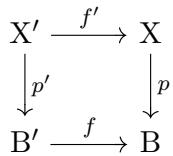
\includegraphics[keepaspectratio]{images/part001_50963eb1.jpg}}

the map p' is strict.

A universally strict map is strict. With the notation of Definition 6, if \(p\) is universally strict, then \(p'\) is universally strict as well. This follows immediately from the definition.

COROLLARY. --- An open map, a proper map, and a map having a continuous local section are universally strict.

Example. --- Let B be a topological space and \((\mathrm{A}_{i})_{i\in\mathrm{I}}\) a covering of B; we denote by A the sum space of the family \((\mathrm{A}_{i})_{i\in\mathrm{I}}\), and \(p: A \to B\) the canonical map. The map p is universally strict under each of the following two hypotheses:

\begin{enumerate}
\def\labelenumi{(\roman{enumi})}
\item
  For every point \(b \in B\) , there exists \(i \in I\) such that b is an interior point of \(A_{i}\) ;
\item
  The family \((A_{i})\) is locally finite and the \(A_{i}\) are closed subsets of B.
\end{enumerate}

Under hypothesis (i), the map p has a continuous section in a neighborhood of every point. Under hypothesis (ii), the map p is proper by definition of the sum space (resp. by TG, I, p. 6, prop. 4 and TG, I, p. 75, th. 1). It is therefore universally strict.

Remark. --- A closed map is not necessarily universally strict (cf. TG, I, p. 96, exerc. 6).

PROPOSITION 11. --- Let

\pandocbounded{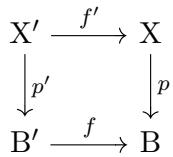
\includegraphics[keepaspectratio]{images/part001_02f1b349.jpg}}

a Cartesian square.

\begin{enumerate}
\def\labelenumi{\alph{enumi})}
\item
Suppose f is strict and surjective. Then, if p' is open (resp. closed, resp. proper), so is p.
\item
Suppose f is closed and surjective. If p' is strict, then p is strict.
\item
Suppose f is universally strict. If p' is universally strict, then p is universally strict.
\end{enumerate}

Note first that for every subset A of X, we have

\[
p ^ {\prime} ((\stackrel {- 1} {f ^ {\prime}}) (\mathrm{A})) = \stackrel {- 1} {f} (p (\mathrm{A})).\tag{20}
\]

Indeed, if \(x' \in (f')^{-1}(\mathrm{A})\), then \(f(p'(x')) = p \circ f'(x') \in p(\mathrm{A})\). Conversely, if \(b' \in f^{-1}(p(\mathrm{A}))\), let \(x \in A\) be such that \(f(b') = p(x)\). By definition of a Cartesian square, there exists a unique \(x' \in X'\) such that \(f'(x') = x\) and \(p'(x') = b'\), so that \(b' \in p'((f')^{-1}(\mathrm{A}))\).

Suppose that f is an open map and \(p'\) is a strict map.

The set \((f')^{-1}(\mathrm{A})\) is open (resp. closed) in \(\mathrm{X}'\). Consequently, the set \(p'((f')^{-1}(\mathrm{A}))\) is open (resp. closed) in \(\mathrm{B}'\). By relation (20), it is also saturated for the equivalence relation defined by \(f\). Since the map \(f\) is assumed to be surjective, we then have \(p(\mathrm{A}) = f(p'((f')^{-1}(\mathrm{A})))\), and since it is strict, the set \(p(\mathrm{A})\) is open (resp. closed) in B. The map \(p\) is therefore open (resp. closed).

For a continuous map to be proper, it is necessary and sufficient that it be closed and that its fibers be quasi-compact (TG, I, p. 75, th. 1). If the map \(p'\) is proper, the map \(p\) is closed by what precedes. Let us study its fibers: if \(b \in B\), let \(b' \in B'\) be such that \(f(b') = b\). By the corollary of I, p. 10, the map \(f'\) induces a homeomorphism \(X_{b'}' \to X_b\). Since \(p'\) is proper, \(X_{b'}'\) is quasi-compact, hence \(X_b\) is also. The map \(p\) is therefore proper.

Let us prove b) and c). Set \(Y = p(X)\) and \(Y' = p'(X')\). Relation (20) applied to X implies that \(Y' = f^{-1}(Y)\). Let g denote the map from \(Y'\) into Y induced by f. In case b), the map g is strict by Remark 1, I, p. 18. In case c), it is strict by Definition 6 since the square

\pandocbounded{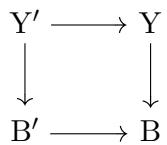
\includegraphics[keepaspectratio]{images/part001_f35053b2.jpg}}

is Cartesian.

Denote by \(q\) and \(q'\) the maps from X to Y and from \(X'\) to \(Y'\), respectively, induced by the maps \(p\) and \(p'\).

\[
\begin{array}{c} \mathrm {X^ {\prime}} \xrightarrow {f ^ {\prime}} \mathrm{X} \\ \Big \downarrow q ^ {\prime} \\ \mathrm {Y^ {\prime}} \xrightarrow {g} \mathrm{Y} \end{array}
\]

Since \(f\) is surjective, \(f'\) is also surjective; by Proposition 9 b), \(p\) is strict.

COROLLARY 1. --- Suppose that the map f is universally strict and surjective and that the map p' is universally strict. Then the map p is universally strict.

Let

\[
\begin{array}{c} \mathrm{Y} \xrightarrow {g ^ {\prime}} \mathrm{X} \\ \Biggl \downarrow q \\ \mathrm{C} \xrightarrow {g} \mathrm{B} \end{array}
\]

a Cartesian square; the goal is to prove that the map q is strict. By Remark 3 of I, p. 16, the squares

\[
\begin{array}{c} \mathrm {X^ {\prime}} \times_ {\mathrm{X}} \mathrm{Y} \xrightarrow {\mathrm{pr} _ {1}} \mathrm {X^ {\prime}} \\ \Biggl \downarrow r \\ \mathrm {B^ {\prime}} \times_ {\mathrm{B}} \mathrm{C} \xrightarrow {\mathrm{pr} _ {1}} \mathrm {B^ {\prime}} \end{array}
\]

and

\[
\begin{array}{c} \mathrm {X^ {\prime} \times_ {X} Y\xrightarrow {pr_ {2}} Y} \\ \Big \downarrow r \\ \mathrm {B^ {\prime} \times_ {B} C\xrightarrow {pr_ {2}} C} \end{array}\tag{21}
\]

are Cartesian, where \(r \colon X' \times_{X} Y \to B' \times_{B} C\) denotes the map induced by \((p', q)\). As the map \(f\) is universally strict and surjective, the same holds for the map \(\mathrm{pr}_2 \colon B' \times_{B} C \to C\) (I, p. 20, def. 6 and I, p. 10, cor. of prop. 4). On the other hand, the map \(r\) is strict, since \(p'\) is assumed to be universally strict. By Proposition 11, c) applied to the Cartesian square (21), the map \(q\) is strict.

COROLLARY 2. --- Let B and X be topological spaces and let \(p\colon X \to B\) be a continuous map. Let \((A_i)_{i \in I}\) be a family of subsets of B that is an open cover of B, or else a locally finite closed cover of B. If for every \(i \in I\), the map \(p_{A_i}\colon \overline{p}^1(A_i) \to A_i\) is strict (resp. universally strict), the map p is strict (resp. universally strict).

For every \(i \in \mathrm{I}\), set \(\mathrm{Y}_i = \overline{p}^{1}(\mathrm{A}_i)\) and \(p_i = p_{\mathrm{A}_i}\). Let A be the sum space of the family \((\mathrm{A}_i)_{i \in \mathrm{I}}\) and Y the sum space of the family \((\mathrm{Y}_i)_{i \in \mathrm{I}}\); let us denote by \(f: \mathrm{A} \to \mathrm{B}\) (resp. \(g: \mathrm{Y} \to \mathrm{X}\), \(q: \mathrm{Y} \to \mathrm{A}\)) the map induced by the family of canonical injections \(A_i \rightarrow B\) (resp. of canonical injections \(Y_i \rightarrow X\) and of the maps \(p_i\)). The square

\[
\begin{array}{c} \mathrm{Y} \xrightarrow {g} \mathrm{X} \\ \Big \downarrow q \\ \mathrm{A} \xrightarrow {f} \mathrm{B} \end{array}
\]

is a Cartesian square (Examples, I, p. 10 and p. 14). By the corollary, I, p. 20, the map \(f\) is universally strict. By Proposition 11, it therefore suffices to prove that the map \(q\) is strict (resp. universally strict) if the maps \(p_i\), for \(i \in I\), are strict (resp. universally strict). We are thus reduced to proving the corollary when the sets \(A_i\), \(i \in I\), form a partition of the space B into open and closed parts, which we will henceforth assume.

Suppose that each of the maps \(p_i\), \(i \in I\), is strict. If U is an open subset of X and is saturated for the equivalence relation defined by p, the set \(p_i(\mathrm{X}_i \cap \mathrm{U})\) is open in \(\mathrm{A}_i\) and \(p(\mathrm{U}) = \bigcup_{i \in \mathrm{I}} p_i(\mathrm{X}_i \cap \mathrm{U})\) is open in B. The map p is therefore strict.

Suppose now that each of the maps \(p_{i}, i \in I\), is universally strict, and let us show that the map p is universally strict. Let C be a topological space and \(h: C \to B\) a continuous map. The goal is to show that the map \(pr_{1}: X \times_{B} C \to C\) is strict. The space C is identified with the sum space of the family \(C_{i} = h^{-1}(A_{i})\), and the space \(X \times_{B} C\) is identified with the direct sum space of the family \(X \times_{B} C_{i} = X_{i} \times_{A_{i}} C_{i}\). Since \(p_{i}\) is universally strict, the map \(pr_{1}: X_{i} \times_{A_{i}} C_{i} \to C_{i}\) is strict. By the preceding, the map \(pr_{1}: X \times_{B} C \to C\) is strict. This proves that the map p is universally strict.

